%%%%%%%%%%%%%%%%%%% vorlage.tex %%%%%%%%%%%%%%%%%%%%%%%%%%%%%
%
% LaTeX-Vorlage zur Erstellung von Projekt-Dokumentationen 
% im Fachbereich Informatik der Hochschule Trier
%
% Basis: Vorlage svmono des Springer Verlags
%
%%%%%%%%%%%%%%%%%%%%%%%%%%%%%%%%%%%%%%%%%%%%%%%%%%%%%%%%%%%%%
\documentclass[envcountsame,envcountchap, deutsch]{i-studis}

\usepackage{makeidx}         	% Index
\usepackage{multicol}        	% Zweispaltiger Index
%\usepackage[bottom]{footmisc}	% Erzeugung von Fu�noten

%%-----------------------------------------------------
%\newif\ifpdf
%\ifx\pdfoutput\undefined
%\pdffalse
%\else
%\pdfoutput=1
%\pdftrue
%\fi
%%--------------------------------------------------------
%\ifpdf
\usepackage[pdftex]{graphicx}
\usepackage{epstopdf}
\usepackage[pdftex,plainpages=false]{hyperref}
%\else
%\usepackage{graphicx}
%\usepackage[plainpages=false]{hyperref}
%\fi

%%-----------------------------------------------------
\usepackage{color}				% Farbverwaltung
%\usepackage{ngerman} 			% Neue deutsche Rechtsschreibung
\usepackage[english, ngerman]{babel}
%\usepackage[latin1]{inputenc} 	% Ermöglicht Umlaute-Darstellung
\usepackage[utf8]{inputenc}  	% Ermöglicht Umlaute-Darstellung unter Linux (je nach verwendetem Format)

%-----------------------------------------------------
\usepackage{listings} 			% Code-Darstellung
\lstset
{
	basicstyle=\scriptsize, 	% print whole listing small
	keywordstyle=\color{blue}\bfseries,
								% underlined bold black keywords
	identifierstyle=, 			% nothing happens
	commentstyle=\color{red}, 	% white comments
	stringstyle=\ttfamily, 		% typewriter type for strings
	showstringspaces=false, 	% no special string spaces
	framexleftmargin=7mm, 
	tabsize=3,
	showtabs=false,
	frame=single, 
	rulesepcolor=\color{blue},
	numbers=left,
	linewidth=146mm,
	xleftmargin=8mm
}
\usepackage{textcomp} 			% Celsius-Darstellung
\usepackage{amssymb,amsfonts,amstext,amsmath}	% Mathematische Symbole
\usepackage[german, ruled, vlined]{algorithm2e}
\usepackage[a4paper]{geometry} % Andere Formatierung
\usepackage{bibgerm}
\usepackage{array}
\hyphenation{ Ele-men-tar-ob-jek-te  ab-ge-tas-tet Aus-wer-tung House-holder-Matrix Le-ast-Squa-res-Al-go-ri-th-men} 		% Weitere Silbentrennung bei Bedarf angeben
\setlength{\textheight}{1.1\textheight}
\pagestyle{myheadings} 			% Erzeugt selbstdefinierte Kopfzeile
\makeindex 						% Index-Erstellung


%--------------------------------------------------------------------------
\begin{document}
%------------------------- Titelblatt -------------------------------------
\title{Implementierung einer Enterprise Search Engine für das \\ Dietrich Online Projekt}
\subtitle{ Implementation of an enterprise search engine for the \\ Dietrich Online project }
%---- Die Art der Dokumentation kann hier ausgewählt werden---------------
%\project{Bachelor-Projektarbeit}
\project{Bachelor-Abschlussarbeit}
%\project{Master-Projektstudium}
%\project{Master-Abschlussarbeit}
%\project{Seminar zur Vorlesung ...}
%\project{Hausarbeit zur Vorlesung ...}
%--------------------------------------------------------------------------
\supervisor{Professor Doktor Christoph Schmitz} 		% Betreuer der Arbeit
\author{ Florian Reitz } 							% Autor der Arbeit
\address{Trier, den 15.10.2019} 							% Im Zusammenhang mit dem Datum wird hinter dem Ort ein Komma angegeben
\submitdate{15.3.2020} 				% Abgabedatum
%\begingroup
%  \renewcommand{\thepage}{title}
%  \mytitlepage
%  \newpage
%\endgroup
\begingroup
  \renewcommand{\thepage}{Titel}
  \mytitlepage
  \newpage
\endgroup
%--------------------------------------------------------------------------
\frontmatter 
%--------------------------------------------------------------------------
\preface

Diese Arbeit entstand als Abschlussarbeit an der Hochschule Trier in Zusammenarbeit mit der Bibliothek der Universität Trier. 
\newline
\newline
Die Idee zu dieser Arbeit entwickelte sich während meiner Arbeit am Dietrich online Projekt. Ich möchte diese Stelle nutzen, um mich beim Dietrich online Team und vor allem bei Herrn Kock für die Unterstützung zu bedanken.
\newline
\newline
Ein besonderer Dank gilt auch Herrn Professor Schmitz und Herrn Röpke für die Betreuung dieser Arbeit.
\newline
\newline
In dieser Arbeit wird aus Gründen der besseren Lesbarkeit das generische Maskulinum verwendet. Die dabei gewählte Form bezieht sich auf alle Geschlechter des Spektrums. 
\newline
Zudem wird DietrichOnline anstelle Dietrich online für eine bessere Lesbarkeit verwendet.
\newline
\newline
Der Code, der für diese Arbeit erstellt wurde, ist unter: \url{https://seafile.rlp.net/f/a70bebdfa575485a89ab/} zu finden. Das Passwort für den Download ist: Bachelor2020.
\newline
\newline
Trier, 2020
\newline
\noindent Florian Reitz				% Vorwort (optional)
\kurzfassung

%% deutsch
\paragraph*{German}
Diese Arbeit handelt von der Analyse diverser Enterprise-Suchmaschinen für das DietrichOnline-Projekt \ref{dietrichonline}. Dabei wurden die Suchmaschinen nach einer Anforderungsliste untersucht und die verbleibenden Kandidaten für einen Ersteindruck aufgesetzt. 

Nachdem sich für Elasticsearch entschieden wurde, wurde diese in einer Docker-Umgebung aufgesetzt. Dabei wurde auf eine verschlüsselte Kommunikation zwischen den einzelnen Systemen viel Wert gelegt.

Im letzten Teil der Arbeit wurde zudem eine prototypische Implementierung in das DietrichOnline-Projekt vorgenommen. Dafür wurde die Suche, sowie die Auto-Vervollständigung auf die Suchmaschine umgezogen.

%% englisch
\paragraph*{English}

This thesis analyzes various enterprise search-engines for the DietrichOnline project \ref{dietrichonline}. The search-engines were checked via a feature list and four of the remaining search engines were set up for a first impression.

After the decision was made for Elasticsearch, it was set up in a Docker environment. Great importance was attached to encrypted communication between the individual systems.

The last part of this thesis is a prototype implementation of the search engine in the DietrichOnline project. The search and the auto-completion function were set up to use Elasticsearch. 			% Kurzfassung Deutsch/English
\tableofcontents 						% Inhaltsverzeichnis
\listoffigures 							% Abbildungsverzeichnis (optional)
\listoftables 							% Tabellenverzeichnis (optional)
%--------------------------------------------------------------------------
\mainmatter                        		% Hauptteil (ab hier arab. Seitenzahlen)
%--------------------------------------------------------------------------
% Die Kapitel werden in separaten .tex-Dateien abgelegt und hier eingebunden.
\chapter{Einleitung und Problemstellung}

Begonnen werden soll mit einer Einleitung zum Thema, also Hintergrund und Ziel erl�utert werden.

Weiterhin wird das vorliegende Problem diskutiert: Was ist zu l�sen, warum ist es wichtig, dass man dieses Problem l�st und welche L�sungsans�tze gibt es bereits. Der Bezug auf vorhandene oder eben bisher fehlende L�sungen begr�ndet auch die Intention und Bedeutung dieser Arbeit. Dies k�nnen allgemeine Gesichtspunkte sein: Man liefert einen Beitrag f�r ein generelles Problem oder man hat eine spezielle Systemumgebung oder ein spezielles Produkt (z.B. in einem Unternehmen), woraus sich dieses noch zu l�sende Problem ergibt.

Im weiteren Verlauf wird die Problemstellung konkret dargestellt: Was ist spezifisch zu l�sen? Welche Randbedingungen sind gegeben und was ist die Zielsetzung? Letztere soll das
beschreiben, was man mit dieser Arbeit (mindestens) erreichen m�chte.
%\chapter{LaTeX-Bausteine}\label{Stile}

Der Text wird in bis zu drei Ebenen gegliedert:

\begin{enumerate}
  \item Kapitel ( \verb\chapter{Kapitel} ), \index{Kapitel}
  \item Unterkapitel  ( \verb \section{Abschnitt} ) und
  \item Unterunterkapitel  ( \verb \subsection{Unterabschnitte} ).
\end{enumerate}

\section{Abschnitt}\index{Abschnitt}
Text der Gliederungsebene 2.


\subsection{Unterabschnitt} \index{Unterabschnitt}
Text der Gliederungsebene 3.
Text Text Text Text Text Text Text Text Text Text Text Text Text Text Text
Beispiel für Quelltext \index{Quelltext} \\[2 ex]
\noindent
\begin{minipage}{1.0\textwidth} \small
\begin{lstlisting}
	Prozess 1:
	
	Acquire();
		a := 1;
	Release();
	...
	Acquire();
	if(b == 0)
	{					
		c := 3;
		d := a;
	}				
	Release();
\end{lstlisting}
\end{minipage}

\vspace{2cm}
\noindent
\begin{minipage}{1.0\textwidth} \small
\begin{lstlisting}
	Prozess 2:
	
	Acquire();
		b := 1;
	Release();
	...
	Acquire();
	if(a == 0)
	{					
		c := 5;
		d := b;
	}				
	Release();
\end{lstlisting}
\end{minipage}
\vskip 1em

Größere Code-Fragmente sollten im Anhang eingefügt werden.

\section{Abbildungen und Tabellen}

Abbildung\index{Abbildung} und Tabellen\index{Tabelle} werden zentriert eingefügt. Grundsätzlich sollen sie
erst dann erscheinen, nach dem sie im Text angesprochen wurden (siehe Abb. \ref{a1}). Abbildungen und Tabellen (siehe Tabelle \ref{t1}) können
im (fließenden) Text (\verb here ), am Seitenanfang (\verb top ), am Seitenende
(\verb bottom ) oder auch gesammelt auf einer nachfolgenden Seite (\verb page )
oder auch ganz am Ende der Ausarbeitung erscheinen. Letzteres sollte man nur
dann wählen, wenn die Bilder günstig zusammen zu betrachten sind und die
Ausarbeitung nicht zu lang ist ($< 20$ Seiten).

\begin{figure} %[hbtp]
	\centering
		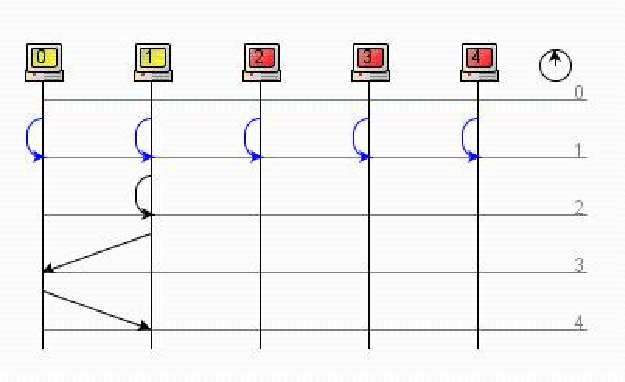
\includegraphics{images/p1ReadSeq.pdf}
	\caption{Bezeichnung der Abbildung}
	\label{a1}
\end{figure}

\begin{table} %[hbtp]
	\centering
		\begin{tabular}{l | l l l l}
		\textbf{Prozesse} & \textbf{Zeit} $\rightarrow$ \\
		\hline
			$P_{1}$ & $W(x)1$ \\
			$P_{2}$ & & $W(x)2$ \\
			$P_{3}$ & & $R(x)2$ & & $R(x)1$\\
			$P_{4}$ & & & $R(x)2$ & $R(x)1$\\
		\end{tabular}
	\caption{Bezeichnung der Tabelle}
	\label{t1}
\end{table}


\section{Mathematische Formel}\index{Formel}
Mathematische Formeln bzw. Formulierungen können sowohl im
laufenden Text (z.B. $y=x^2$) oder abgesetzt und zentriert im Text
erscheinen. Gleichungen sollten für Referenzierungen nummeriert
werden (siehe Formel \ref{gl-1}).
\begin{equation}
\label{gl-1}
e_{i}=\sum _{i=1}^{n}w_{i}x_{i}
\end{equation}

Entscheidungsformel:

\begin{equation}
\psi(t)=\left\{\begin{array}{ccc}
1 &  \qquad 0 <= t < \frac{1}{2} \\
-1 &  \qquad \frac{1}{2} <= t <1 \\
0 & \qquad sonst
\end{array} \right.
\end{equation}


Matrix:\index{Matrix}
\begin{equation}
A = \left(
\begin{array}{llll}
a_{11} & a_{12} & \ldots & a_{1n} \\
a_{21} & a_{22} & \ldots & a_{2n} \\
\vdots & \vdots & \ddots & \vdots \\
a_{n1} & a_{n2} & \ldots & a_{nn} \\
\end{array}
\right)
\end{equation}

Vektor:\index{Vektor} 

\begin{equation}
\overline{a} = \left(
\begin{array}{c}
a_{1}\\
a_{2}\\
\vdots\\
a_{n}\\
\end{array}
\right)
\end{equation}

\section{Sätze, Lemmas und Definitionen}\index{Satz}\index{Lemma}\index{Definition}

Sätze, Lemmas, Definitionen, Beweise,\index{Beweis} Beispiele\index{Beispiel} können in speziell dafür vorgesehenen Umgebungen erstellt werden.

\begin{definition}(Optimierungsproblem)

Ein \emph{Optimierungsproblem} $\mathcal{P}$ ist festgelegt durch ein Tupel
$(I_\mathcal{P}, sol_\mathcal{P}, m_\mathcal{P}, goal)$ wobei gilt

\begin{enumerate}
\item $I_\mathcal{P}$ ist die Menge der Instanzen,
\item $sol_\mathcal{P} : I_\mathcal{P} \longmapsto \mathbb{P}(S_\mathcal{P})$ ist eine Funktion, die jeder Instanz $x \in I_\mathcal{P}$ eine Menge zulässiger Lösungen zuweist,
\item $m_\mathcal{P} : I_\mathcal{P} \times S_\mathcal{P} \longmapsto \mathbb{N}$ ist eine Funktion, die jedem Paar $(x,y(x))$ mit $x \in I_\mathcal{P}$ und $y(x) \in sol_\mathcal{P}(x)$ eine
Zahl $m_\mathcal{P}(x,y(x)) \in \mathbb{N}$ zuordnet (= Maß für die Lösung $y(x)$ der Instanz $x$), und
\item $goal \in \{min,max\}$.
\end{enumerate}

\end{definition}

\begin{example} MINIMUM TRAVELING SALESMAN (MIN-TSP)
\begin{itemize}
\item $I_{MIN-TSP} =_{def}$ s.o., ebenso $S_{MIN-TSP}$
\item $sol_{MIN-TSP}(m,D) =_{def} S_{MIN-TSP} \cap \mathbb{N}^m$ 
\item $m_{MIN-TSP}((m,D),(c_1, \ldots , c_m)) =_{def} \sum_{i=1}^{m-1} D(c_i, c_{i+1}) + D(c_m,c_1)$ 
\item $goal_{MIN-TSP} =_{def} min$
\end{itemize}
\begin{flushright}
$\qed$
\end{flushright}
\end{example}

\begin{theorem} Sei $\mathcal{P}$ ein \textbf{NP}-hartes Optimierungsproblem.
Wenn $\mathcal{P} \in$ \textbf{PO}, dann ist \textbf{P} = \textbf{NP}.
\end{theorem}

\begin{proof} Um zu zeigen, dass \textbf{P} = \textbf{NP} gilt, genügt es
wegen Satz A.30 zu zeigen, dass ein einziges \textbf{NP}-vollständiges
Problem in \textbf{P} liegt. Sei also $\mathcal{P}'$ ein beliebiges \textbf{NP}-vollständiges Problem.

Weil $\mathcal{P}$ nach Voraussetzung \textbf{NP}-hart ist, gilt insbesondere
$\mathcal{P}' \leq_T \mathcal{P}_C$. Sei $R$ der zugehörige
Polynomialzeit-Algorithmus dieser Turing-Reduktion.
Weiter ist $\mathcal{P} \in$ \textbf{PO} vorausgesetzt, etwa vermöge eines
Polynomialzeit-Algorithmus $A$. Aus den beiden
Polynomialzeit-Algorithmen $R$ und $A$ erhält man nun
leicht einen effizienten Algorithmus für $\mathcal{P}'$: Ersetzt man
in $R$ das Orakel durch $A$, ergibt dies insgesamt eine polynomielle
Laufzeit. 
%\begin{flushright}
$\qed$
% \end{flushright}
\end{proof}

\begin{lemma} Aus \textbf{PO} $=$ \textbf{NPO} folgt \textbf{P} $=$ \textbf{NP}.
\end{lemma}

\begin{proof} Es genügt zu zeigen, dass unter der angegeben
Voraussetzung KNAPSACK $\in$ \textbf{P} ist.

Nach Voraussetung ist MAXIMUM KNAPSACK $\in$ \textbf{PO},
d.h. die Berechnung von $m^*(x)$ für jede Instanz $x$ ist
in Polynomialzeit möglich. Um KNAPSACK bei Eingabe
$(x,k)$ zu entscheiden, müssen wir nur noch $m^*(x) \geq k$
prüfen. Ist das der Fall, geben wir $1$, sonst $0$ aus. Dies
bleibt insgesamt ein Polynomialzeit-Algorithmus. 
\begin{flushright}
$\qed$
\end{flushright}
\end{proof}

\section{Fußnoten}

In einer Fußnote können ergänzende Informationen\footnote{Informationen die für die Arbeit zweitrangig sind, jedoch für den Leser interessant sein könnten.} angegeben werden. Außerdem kann eine Fußnote auch Links enthalten. Wird in der Arbeit eine Software (zum Beispiel Java-API\footnote{\url{http://java.sun.com/}}) eingesetzt, so kann die Quelle, die diese Software zur Verfügung stellt in der Fußnote angegeben werden.

\section{Literaturverweise}\index{Literatur}
Alle benutzte Literatur wird im Literaturverzeichnis angegeben\footnote{Dazu wird ein sogennanter bib-File, literatur.bib verwendet.}. Alle angegebene Literatur sollte mindestens einmal im Text referenziert werden.
\chapter{Vergleich der Enterprise Search Engines}

In ersten Schritt werden diverse Enterprise Search Engines evaluiert. Dafür wurde eine Anforderungsliste mit den Mitarbeitern erstellt. Die Systeme welche bei diesen Vergleich nach Features am besten abschneiden werden anschließend aufgesetzt, getestet und genauer verglichen.

\begin{itemize}
    \item Open Source oder Kostenlos
    \item Unterstützung von Facetten
    \item Ranking der Suchergebnisse
    \item Volltextsuche
    \item Support für PDF, SQL, XML
    \item Logging-Möglichkeit
\end{itemize}

Des Weiteren sind die folgenden Funktionen auch wichtig, allerdings keine K.O. Kriterien:

\begin{itemize}
    \item Support für PostgreSQL
    \item Backup Funktionen
    \item Auto-Korrektur und Auto-Vervollständigung
    \item Security Features
    \item PHP-Support
    \item bezahlter Support
\end{itemize}

Durch die begrenzten finanziellen Mittel und die lange Projektlaufzeit besteht die Notwendigkeit eine kostenfreie, im besten Fall sogar Open Source Suchmaschine zu finden. Auch äußerst wichtig ist der Support für Facetten, da viele Dietrich-Online als Suchmaschine den Nutzer einige Tools zum Verfeinern seiner Suchergebnisse zur Verfügung stellen will. Das Ranking der Suchergebnisse ist vor allem für die Transparenz wichtig, da hier mit vielen Daten gearbeitet wird, welche allerdings nicht alle gleichzeitig dargestellt werden können. Dieses Problem kann mit einer Gewichtung der Suchergebnisse behoben werden, welches dann auf der Seite für Transparenz veröffentlicht wird. Die Volltextsuche wird es möglich machen auch nach Schlüsselwörtern im Titel zu suchen. Der Support von den verschiedenen Dateiformaten ergibt sich dadurch, dass dieses Projekt stark gewachsen ist. Es gibt viele Prozessschritte, welche auf denselben Daten in verschiedenen Formen arbeiten. Darunter werden alle Einträge im XML Format bearbeitet, es gibt alle Scans als PDF und für die Webseite sind alle Daten nochmals in der Datenbank vorhanden. Dadurch gibt sich auch das Problem, dass Daten mehrfach vorliegen welches sicherlich Später von größerer Bedeutung sein wird. Als letztes ist es noch wichtig, dass eine Logging-Möglichkeit geboten wird, damit schnell und effizient Probleme mit dem System erkannt und gelöst werden können.

Ein Support für PostgreSQL ist für dieses Projekt nicht so wichtig, allerdings könnte es sein, dass der Server später auch andere Datenbanken verwaltet. Der Server wird sowieso täglich durch einen Automatismus gesichert. Allerdings ist eine manuelle Backup-Lösung wünschenswert, um die Suchmaschine losgelöst von den Server zu sichern und gegebenenfalls auch einfach auf einen anderen Server umzuziehen. Auto-Korrektur und Auto-Vervollständigung sind beide sehr interessant, um den Nutzer mehr Komfort-Funktionen bieten zu können. Der Server sollte ja generell nur intern Ansprechbar sein. Allerdings gibt es für manche der Suchmaschinen eine Web-Oberfläche, da wäre es wichtig eine sichere Verbindung dorthin und gegebenenfalls eine Möglichkeit der Mehrfaktor-Authentifizierung zu haben. Einen PHP-Connector, welcher Objekte zum Umgang mit der Suchmaschine bietet, wäre wünschenswert. Allerdings bieten einige Suchmaschinen auch die Möglichkeit über JSON Anfragen an die Suchmaschine zu stellen. Allerdings sollte zumindest eine der beiden Möglichkeiten gegeben sein. Zuletzt wäre für akute Probleme ein bezahlter Support, der dafür schneller reagiert wünschenswert. 

\section{Apache Lucene Core}
\label{lucenecore}

Lucene Core ist eine Open Source Enterprise Search Engine von der Apache Foundation geschrieben in Java.

Das Lucene Projekt wurde im Jahre 1997 vom Entwickler Doug Cutting gestartet. 2001 ist es dann der Apache Foundation als Teil des Jakarta-Projekts beigetreten und wurde 2005 ein eigenes Hauptprojekt der Foundation. \cite{Wikipedia.2019c}

Lucene Core erfüllt alle der Grundanforderungen. Für das Monitoring gibt es eine Klasse, die es auch ermöglicht, dass langsame Query’s geloggt werden. Zudem bietet es Support für PostgreSQL und Auto-Korrektur/Auto-Vervollständigung. Da es keine Web-Oberfläche besitzt, gibt es auch keine weiteren Sicherheitsfunktionen. Einen PHP-Connector gibt es leider auch nicht, man müsste daher mit PHP direkte Systemaufrufe an Java machen. Bezahlten Support gibt es hier nicht, da dieses Projekt zur Apache Foundation gehört. 
\cite{TheApacheSoftwareFoundation.2019b}

\section{Terrier}
\label{terrier}

Terrier ist eine Open Source Enterprise Search Engine geschrieben in Java. Entwickelt und gepflegt wird diese von der University of Glasgow. Sie existiert bereit seit 10 Jahren und besitzt, laut Webseite, eine breite Nutzerbasis. 
Terrier erfüllt leider nicht alle Grundanforderungen, da es keine direkte Möglichkeit gibt SQL zu indexieren. Es gibt allerdings eine Möglichkeit das SQL in JSON zu konvertieren und dieses dann in die Suchmaschine einzupflegen. Auch scheint es kein Support für Facetten gegeben.
\cite{McCreadie.2019}

\section{Sphinx}
\label{sphinx}

Sphinx ist eine Suchmaschine entwickelt von Andrew Aksyonoff. Das Akronym steht für „SQL Phrase Index“.\cite{SphinxTechnologiesInc.b} Bis zur Version 2 wurde sie aktiv Open Source entwickelt. Ab Version 3 wurde die Entwicklung closed Source. Auf der Github-Seite steht: „The sources for 3.0 will also be posted here when we decide to make those publicly available.“ \cite{sphinxserach.2019}, also gibt es kein genaues Datum ob und wann die Version 3 Open Source geht. Version 3.1.1 wurde im Oktober 2018 veröffentlicht und seitdem lässt sich auch nichts mehr über das Projekt finden. Von daher ist davon auszugehen, dass das Projekt nicht mehr weitergeführt wird. 

Zu den Features ist festzuhalten, dass es keinen nativen PDF-Support in der Open-Source Version existiert, ab der Version 3 jedoch wurde ein Dokumenten-Speicher eingebaut. Allerdings werden die anderen Anforderungen alle erfüllt. Es existiert, laut Webseite, sogar ein bezahlter Support, allerdings ist fraglich, ob man mit der Firma noch in Kontakt treten kann. \cite{SphinxTechnologiesInc.2019}

\section{Apache Solr}
\label{solr}

Apache Solr ist eine, auf Lucene Core \ref{lucenecore} viel eingesetzte Search Engine von der Apache Foundation. Sie basiert auf Apache Lucene Core und erweitert dieses um ein grafische Benutzeroberfläche und einige Features. 
Die Entwicklung dafür begann 2004 als ein internes Projekt von CNET um eine bessere Suche für die eigene Webseite zu bieten. Später im Jahre 2006 hat CNET dann den Source Code an die Apache Foundation weitergegeben. Dadurch wurde  es zu einem eigenen Projekt bei der Apache Foundation. Im Jahre 2009 wurden Solr dann in das Apache Lucene Projekt eingefügt. Dort wird es auch aktuell noch weiterentwickelt. \cite{Wikipedia.2019b}

Solr wird unter anderem von DuckDuckGo und Best Buy eingesetzt. Durch die Unterstützung von der Apache Foundation längerfristige Weiterentwicklung abzusehen. 

Da Solr zur Apache Foundation gehört, ist es Open Source. Es bietet viele Funktionen von Haus, damit erfüllt es alle Grundanforderungen und besitzt darüber hinaus auch Support für fast alle Bonus-Features. Einzig und allein gibt es keinen bezahlten Support, dafür allerdings eine große Community, welche man durch einen Mailing Liste oder IRC erreichen kann.

\cite{TheApacheSoftwareFoundation.2019}

\section{ElasticSearch}
\label{elasticsearch}

Eine weitere großes Enterprise Search Engine ist ElasticSearch. Auch dieses Projekt arbeitet auf der Basis von Lucene. Zu den bekanntesten Kunden zählen Ebay und Adobe. Gestartet wurde das Projekt in den jungen 2000ern von Shay Banon, um eine Verwaltung für die Rezepte seiner Frau zu schaffen. Im Juni 2012 haben sich dann Logstash, ein Logging Dienst, Kibana, ein UI für ElasticSearch, und ElasticSearch zusammengetan. Alle kamen zusammen in der ElasticSearch Incorporated. Seitdem wurden der Produktkatalog stetig erweitert und die Produkte weiterentwickelt. Viele der weiteren Produkte sind allerdings nicht mehr Open-Source oder kostenlos. Der ELK-Stack ist allerdings weiterhin kostenlos und ElasticSearch zudem auch als Open-Source Variante zu haben. Eine genauere Aussage, welche Features nur in der kostenlosen und nicht in der Open-Source Variante zu finden sind, finden sich in der Tabelle \ref{vglTable}.

ElasticSearch erfüllt alle der Grundanforderungen, auch in der Open-Source Variante. Auch viele der optionalen Features kann man in der Open Source Variante genießen. Einzig die Sicherheitsfunktionen, wie rollen-basierte Authentifizierung sind der kostenlosen Variante vorbehalten. Eine Möglichkeit auf bezahlten Support besteht auch, dafür muss auf eine bezahlte Version gewechselt werden, was auch einige Funktionen wie IP-Filter mit sich bringt. Allerdings ist diese daraufhin auch nichtmehr Open-Source. \cite{Elasticsearch.2019}

\section{Fess}
\label{fess}

Fess ist eine Enterprise Search Engine basierend auf ElasticSearch entwickelt von dem japanischen Unternehmen CodeLibs. Die Suchmaschine ist komplett Open-Source und wird unter der Apache-Lizenz entwickelt.

Die Suchmaschine erfüllt alle Grundanforderungen. Darüber hinaus bietet es Support für PostgreSQL, Backups (sogar über die Web-Oberfläche) und Auto-Korrektur und Vervollständigung. Es gibt keinen direkten PHP Support, allerdings können anfragen über JSON geschickt werden. Ein bezahlter Support ist auch möglich über die Firma N2SM Incorporated. \cite{N2SM.2019} Bei dieser Arbeiten anscheinend auch einige der Entwickler von FESS. Sicherheitsfunktionen werden über rollen-basierte Authentifizierung mitgeliefert. \cite{CodeLibs.2019}

\section{Algolia}
\label{algolia}

Algolia ist eine cloud-basierte Search Engine, welche unter anderem von Twitch und Lacoste verwendet wird. Die Suchmaschine wird hierbei als SAAS (Software as a Service) angeboten.  Hierbei lädt man die Daten auf Algolia Server und dann daraufhin der API Suchen auf den Daten ausführen.

Es erfüllt alle Grundanforderungen, wobei allerdings in der kostenlosen Variante grade einmal 10 Tausend Einträge und 50 Tausend Operationen im Monat erlaubt sind. Diese Einschränkung macht die kostenlose Variante dieser Suchmaschine für das Dietrich-Online Projekt unbrauchbar. Von den optionalen Anforderungen erfüllt Algolia auch alle. Der bezahlte Support wird ab der Starter Edition für 30 Dollar im Monat mitgeliefert. \cite{Algolia.2019}

\section{Manticore Search}
\label{manticore}

Manticore Search Engine ist eine Open-Source Solution basierend auf Sphinx \ref{sphinx}. Nachdem Sphinx Closed-Source gegangen ist, wurde auf der letzten offenen Version die erste Version von Manticore Search entwickelt. Zu den großen Kunden zählen unter anderem Craigslist und Boardreader.

Manticore erfüllt fast alle Grund Anforderungen, allerdings ist kein nativer PDF-Support gegeben. Es muss daher auf eine Konvertierung der Daten auf XML gesetzt werden. Es findet sich außerdem eine Unterstützung von PostgreSQL, sowie Auto-Korrektur und Vervollständigung. Es gibt auch einen Query-Log. Zuletzt gibt es noch eine Option auf bezahlten Support. Die Supportkosten sind dabei direkt auf der Webseite angegeben und belaufen sich auf 3000 Dollar im Jahr für den Standard Support. \cite{ManticoreSoftwareLtd.2019}

\section{Xapian}
\label{xapian}

Xapian ist eine Open-Source Enterprise Suchmaschine, welche von Zeit-Online, der Universitätsbibliothek Köln und der Debian Webseite genutzt wird. Die Suchmaschine basiert auf Open Muscat, einer Suchmaschine, welche an der Cambridge Universität in den 1980ern von Dr. Martin Porter entwickelt wurde. In 2001, als Open Muscat Closed-Source ging, haben sich einige Entwickler die letzte offene Version geladen und diese weiterentwickelt.

Sie erfüllt alle der Grundanforderungen, wenn auch Logging nur im Grundsinne erfüllt wird, da nur Errors geschmissen werden. Des Weiteren bietet die Suchmaschine Support für PostgreSQL. Auch eine Replikations-Funktion wird mitgeliefert. Sie bietet auch Auto-Korrektur und Auto-Vervollständigung. Ein Login-System mit Sicherheitsfunktionen gibt es durch das Fehlende Frontend Administration nicht. Es gibt allerdings die Möglichkeit mit Omega eine CGI-Suche zu nutzen. Diese Suche bietet allerdings keine Administration, sondern nur eine grafische Oberfläche für Suchanfragen.

Auch gibt es eine Möglichkeit für bezahlten Support. Auf der Webseite werden zwei Firmen angegeben, welche bezahlten Support bieten. Allerdings funktioniert der Link aktuell nur für eine der beiden Firmen aktuell. Zudem ist ein PHP-Connector für die Suchmaschine vorhanden, was die Einbindung ist das Projekt vereinfacht. \cite{XAP.2019}

\section {Vorauswahl}

Alle Suchmaschinen die zumindest die Grundanforderungen erfüllen, werden hier in der Tabelle nun nochmals aufgeführt für einen leichteren Vergleich. 

\begin{table} %[hbtp]
	\centering
		\begin{tabular}{l | l | l | l | l | l | l | l}
		& \textbf{LC} & \textbf{SH} & \textbf{AS} & \textbf{ES}  & \textbf{FE} & \textbf{AG} & \textbf{XP} \\
        \hline
        Open Source oder Kostenlos                  & x & x  & x & x  & x & x  & x  \\
        Unterstützung von Facetten                  & x & x  & x & x  & x & x  & x  \\
        Ranking der Suchergebnisse                  & x & x  & x & x  & x & x  & x  \\
        Volltextsuche                               & x & x  & x & x  & x & x  & x  \\
        Support für PDF, SQL, XML                   & x & x* & x & x  & x & x  & x  \\
        Monitoring / Logging                        & x & x  & x & x  & x & x  & x? \\
        \hline
        Support für PostgreSQL                      & x & x  & x  & x  & x & x  & x \\
        Backup                                      & - & -  & x  & x  & x & x+ & - \\
        Auto-Korrektur und Vervollständigung        & x & x  & x  & x  & x & x  & x \\
        Security Features                           & - & -  & x- & x* & x & x  & - \\
        PHP Support                                 & - & x  & x  & x  & - & x  & x \\
        bezahlter Support                           & - & x  & -  & x  & x & x  & x \\
        \hline
        unter aktiver Entwicklung**                 & x & -  & x  & x  & x & x  & x \\
        offizelles Docker Image                     & - & -  & x  & x  & x & -  & - \\
        Synonym Support                             & x & x  & x  & x  & x & x  & x \\
        Web-Interface                               & - & -  & x  & x  & x & x  & - \\
        Plugin Support                              & - & x  & x  & x  & x & -  & - \\
        JSON oder RESTful API                       & - & x* & x  & x  & x & -  & x-- \\
        SQL-Like Query Support                      & - & x  & x  & x  & - & -  & - \\
		\end{tabular}
    \caption{Feature-Vergleich der verschiedenen Enterprise Suchmaschinen }
    \label{vglTable}

    *  = Feature nur in der kostenlosen Variante verfügbar. \\
    ** = Update innerhalb des letzen halben Jahres \\
    -- = Nur mit Omega CGI installiert \\
    +  = Anbieter kümmert sich um das Feature \\
    -  = Funktion nur per Plugin Implementiert \\

    Die Tabelle vergleicht einige Features der ausgewählten Search Engines. Dabei wurden die Namen aus Platzgründen wie folgt abgekürzt:

    \begin{itemize}
        \item LC = Lucene Core \ref{lucenecore}
        \item SH = Sphinx \ref{sphinx}
        \item AS = Apache Solr \ref{solr}
        \item ES = ElasticSearch \ref{elasticsearch}
        \item FE = Fess \ref{fess}
        \item AG = Algolia \ref{algolia}
        \item XP = Xapian \ref{xapian}
    \end{itemize} 


\end{table}


Nach einem ersten Überblick wurden nun Aufgrund der Auswahlkriterien diese Systeme zum genaueren Vergleich ausgewählt: Apache Solr, Manticore Search, ElasticSearch (in der kostenlosen Version) und Xapian. Lucene Core wird nicht genauer untersucht, da Solr ein umfassenderes Paket bietet, welches den gestellten Anforderungen mehr entspricht.
\chapter{Nutzung des Open Archives Initiative Protokolls für Metadaten}

Das Open Archives Initiative Protocol for Metadata Harvesting (OAI-PMH) ist ein Protokoll zum Austausch von Metadaten. Dabei werden Anfragen per GET oder POST-Request angefragt. Als Antwort erhält man im Folgenden ein XML-Dokument. So können die Metadaten mit bestimmten Facetten abgefragt werden (zum Beispiel Autor). Dabei geht es allerdings darum primär darum Änderungen weiterzugeben. So können durch dieses Protokoll neue Einträge oder Änderungen in der Datenbank weitergeben werden.
\cite{DeutscheNationalBibliothek.2019}

\section{OAI Harverester}

Ein OAI Harverester ist ein Programm, welches durchgehend einen Abgleich der Daten vollführt. Dabei lässt es sich die Änderungen mit einem List-Befehl von dem Server geben und gleicht diese danach mit der eigenen Struktur ab. Sollten dabei Unterschiede festgestellt werden, werden daraufhin die Änderungen auch beim Harverester eingefügt. So steht der Harverester immer mit dem Server auf einen Stand.
\cite{DeutscheNationalBibliothek.2019}

\section{Support der Enterprise Search Engines}

Bei den vorhin genannten Enterprise Search Engines gibt es keine mit nativen OAI Harverester Support. Es gibt die Möglichkeit für manche der Suchmaschinen ein solches Verhalten mithilfe von Plugins zu implementieren. Allerdings sind die meisten dieser Add-ons auch schon veraltet.

\section{Auswertung}

Durch eine fehlende Basisimplementierung des Protokolls in den einzelnen Suchmaschinen und der Möglichkeit eines direkten Zugriffs auf die Datenbank, sehe ich keinen Grund dieses Protokoll zu verwenden. Es müsste ein Server vor die Datenbank installiert werden und ein Harverester vor der ESE. Dies ist ein großer Mehraufwand, welcher bei diesem Anwendungsfall nicht notwendig ist. Sollte allerdings diese Suchmaschine ein übergreifendes System werden, kann darüber nachgedacht werden, die anderen Datenbanken per OAI-Harverester anzusprechen.
\chapter{Zusammenfassung und Ausblick}

Diese Bachelorarbeit hat sich ausführlich mit Enterprise-Suchmaschinen auseinandergesetzt, diese Verglichen und letztendlich eine in das DietrichOnline-Projekt implementiert. Das Ziel dabei war es eine geeignete Suchmaschine für dieses Projekt zu finden und implementieren.  

Im ersten Schritt wurden diverse Suchmaschinen erstmal nach einer Anforderungsliste verglichen. Dafür wurde eine Tabelle erstellt, welche alle Suchmaschinen anhand der gefundenen Funktionen verglichen. Mithilfe dieser Basis wurden vier Suchmaschinen für den genaueren Vergleich herausgesucht.

Für den genaueren Vergleich wurden diese Suchmaschinen nacheinander aufgesetzt und einige Dokumente indexiert. Dabei musste die Suchmaschine selbständig die Daten aus der Datenbank laden und indexieren. Zudem wurde auch die Benutzerfreundlichkeit untersucht. Dafür wurde die Oberfläche, insofern eine vorhanden war, und die Dokumentation bewertet. Zum Schluss wurde daraufhin eine Suchmaschine ausgewählt, welche in das DietrichOnline-Projekt implementiert werden sollte. Dabei war es aufgrund der Zeit leider nicht möglich einen korrekten wissenschaftlichen Vergleich zu erstellen. Es wurde lediglich ein Ersteindruck gewonnen.

Als Nächstes wurde über die Möglichkeit nachgedacht einen OAI Harverester vor die Datenbank zu stellen, um eine normierte Schnittstelle zwischen der Datenbank und Suchmaschine herzustellen. Nach einer kurzen Analyse wurde diese Methodik allerdings verworfen, da ein direkter Zugriff auf die Datenbank möglich ist und somit der Vorgang um an die zu indexierenden Daten zu kommen nur komplizierter gestaltet wird. Diese Funktion könnte allerdings für Datenbanken ohne direkten Zugriff interessant sein. 

Nachdem nun eine Suchmaschine ausgewählt wurde, ging es nun darum diese ordentlich aufzusetzen. Dabei wurde in dieser Arbeit Docker-Compose verwendet. Die Kommunikation zwischen den einzelnen virtuellen Containern wurde hierbei mit selbst generierten Zertifikaten verschlüsselt. Dabei kam es zu einigen Problemen mit der Generierung und Verwendung der Zertifikate, weshalb darüber nachgedacht werden sollte, ob die Verschlüsselung innerhalb des Systems zielführend ist, insofern das System weiterhin auf einen Server laufen soll. 

Im letzten Schritt wurde nun noch eine prototypische Implementierung in das Projekt vorgenommen. Dafür wurde ein Index mit allen für die Suche wichtigen Daten aufgebaut. Um die Größe des Indexes zu minimieren wurde für alle Felder ein vorheriges Mapping vorgenommen. Zudem wurden extra Felder für eine Auto-Vervollständigungsfunktion indexiert. Mithilfe dieses Indexes wurde die Suche für die Nutzer verbessert. Es werden nun mehr verschiedene Sucharten unterstützt. Auch ist es nun möglich mehr als 1001 Ergebnisse zu erhalten. Dies war vorher eine durch die Datenbank auferlegte Grenze. Um zu zeigen, was die Suchmaschine sonst noch für Funktionen unterstützt wurde zudem eine Funktion eingebaut, die die zehn Autoren auflistet, welche die meisten Artikel in der aktuellen Suche geschrieben haben. 

Es wurde für einen Vergleich noch ein Index über alle Lemmata aufgebaut. Dieser ist der aktuell am langsamsten ladende Teil des Projekts. Mit dem Wechsel auf Elasticsearch ist es so gelungen die Laufzeit von dieser Abfrage, um 50 \% zu verringern. 

Zur Implementierung wurde der offizielle Klient von Elasticsearch verwendet, welcher auf einer sehr niedrigen Ebene arbeitet. Es gibt auch Klienten, welche das Level ein wenig mehr abstrahieren und so eine angenehmere Erfahrung bieten, allerdings diese alle nicht offiziell unterstützt. Daher habe ich mich in dieser Arbeit auf den Klienten von Elasticsearch fokussiert. 

Sobald die Suchmaschine in das Projekt eingegliedert ist, können viele weitere Probleme des Projektes gelöst werden. So können zum Beispiel Synonymlisten für Autoren geführt werden, um die verschiedenen Schreibweisen bestimmter Autoren auszugleichen. Auch ist es mit der Suchmaschine möglich dem DDC-Baum, welcher schon seit langer Zeit implementiert werden sollte, leichter einzubauen. Zudem bietet Elasticsearch Funktionen zur Autokorrektur, welche die Sucherfahrung positiv bereichern können. Und für die Entwickler nimmt Elasticsearch einiges an Problemen mit der Datenbank ab. Aktuell werden viele Felder mithilfe von Triggern und Funktionen erstellt. Diese Trigger können nun auf Logstash übertragen werden, um so die Datenbank zu entlasten.

Damit nicht bei jeder Anfrage eine Zertifikats-Autorität mit gereicht werden muss, kann auch noch ein sogenannter Reverse Proxy vor die Elasticsearch Instanz gesetzt werden, welcher daraufhin Zertifikate mithilfe von LetsEncrypt generiert.

% ...
%--------------------------------------------------------------------------
\backmatter                        		% Anhang
%-------------------------------------------------------------------------
\bibliographystyle{geralpha}			% Literaturverzeichnis
\bibliography{literatur}     			% BibTeX-File literatur.bib
%--------------------------------------------------------------------------
\printindex 							% Index (optional)
%--------------------------------------------------------------------------
\begin{appendix}						% Anhänge sind i.d.R. optional
   \chapter{Glossar}

\abbreviation{ESE}{Enterprise Search Engine}
\abbreviation{Facetten}{Filter in Bibliothekarssprache}
\abbreviation{OAI}{Open Archives Initiative}
\abbreviation{OCR}{Optical Character Recognition}
			% Glossar   
   \chapter{Erklärung der Kandidatin / des Kandidaten}

\begin{description}[$\Box$~]
\item[$\Box$] Die Arbeit habe ich selbstständig verfasst und keine anderen als die angegebenen Quellen und Hilfsmittel verwendet.\\
\end{description}

\vspace{2cm}

\begin{minipage}[t]{3cm}
\rule{3cm}{0.5pt}
Datum
\end{minipage}
\hfill
\begin{minipage}[t]{9cm}
\rule{9cm}{0.5pt}
Unterschrift der Kandidatin / des Kandidaten
\end{minipage}	% Selbstständigkeitserklärung
\end{appendix}

\end{document}
